\documentclass[11pt]{article}
% Shared preamble for the Svetoch papers.
% Each paper.tex \input's this file (compile from inside the paper's folder):
%     \documentclass[11pt]{article}
%     % Shared preamble for the Svetoch papers.
% Each paper.tex \input's this file (compile from inside the paper's folder):
%     \documentclass[11pt]{article}
%     % Shared preamble for the Svetoch papers.
% Each paper.tex \input's this file (compile from inside the paper's folder):
%     \documentclass[11pt]{article}
%     \input{../tex/preamble.tex}
% Figures live in ../figures/*.pdf  (graphicspath set below).
\usepackage[utf8]{inputenc}
\usepackage[T1]{fontenc}
\usepackage{lmodern}
\usepackage[a4paper,margin=1in]{geometry}
\usepackage{amsmath,amssymb}
\usepackage{graphicx}
\graphicspath{{../figures/}}
\usepackage{booktabs}
\usepackage{caption}
\captionsetup{font=small,labelfont=bf}
% --- Minimal, siunitx-free unit support (so papers compile on any TeX install) ---
\usepackage{textcomp}
\newcommand{\SI}[2]{#1\,#2}
\newcommand{\si}[1]{#1}
\newcommand{\hertz}{Hz}
\newcommand{\meter}{m}
\newcommand{\centi}{c}
\newcommand{\milli}{m}
\newcommand{\micro}{\textmu}
\newcommand{\second}{s}
\newcommand{\kelvin}{K}
% ---------------------------------------------------------------------------------
\usepackage[colorlinks=true,linkcolor=blue,citecolor=blue,urlcolor=blue]{hyperref}
\usepackage{xcolor}
\definecolor{accent}{HTML}{6366F1}

% Common author block (add affiliation/ORCID if available before publishing)
\newcommand{\svetochauthor}{Oleg Yuryevich Kirichenko \\[4pt]
  \normalsize Independent researcher \\[2pt]
  \normalsize \href{mailto:urevich55@gmail.com}{urevich55@gmail.com} \quad\textbullet\quad GitHub: \href{https://github.com/infosave2007}{@infosave2007}}

\newcommand{\svetochfooter}{%
  \vspace{1em}\noindent\rule{\linewidth}{0.4pt}\\[2pt]
  {\footnotesize Part of the \emph{Svetoch} series (defensive publication, not patented).
  Project and code: \href{https://github.com/infosave2007/svetoch}{github.com/infosave2007/svetoch};
  related VMF/NVG theory: \href{https://github.com/infosave2007/vmf}{github.com/infosave2007/vmf}.
  Released for the public record to establish authorship and priority.}}

% Figures live in ../figures/*.pdf  (graphicspath set below).
\usepackage[utf8]{inputenc}
\usepackage[T1]{fontenc}
\usepackage{lmodern}
\usepackage[a4paper,margin=1in]{geometry}
\usepackage{amsmath,amssymb}
\usepackage{graphicx}
\graphicspath{{../figures/}}
\usepackage{booktabs}
\usepackage{caption}
\captionsetup{font=small,labelfont=bf}
% --- Minimal, siunitx-free unit support (so papers compile on any TeX install) ---
\usepackage{textcomp}
\newcommand{\SI}[2]{#1\,#2}
\newcommand{\si}[1]{#1}
\newcommand{\hertz}{Hz}
\newcommand{\meter}{m}
\newcommand{\centi}{c}
\newcommand{\milli}{m}
\newcommand{\micro}{\textmu}
\newcommand{\second}{s}
\newcommand{\kelvin}{K}
% ---------------------------------------------------------------------------------
\usepackage[colorlinks=true,linkcolor=blue,citecolor=blue,urlcolor=blue]{hyperref}
\usepackage{xcolor}
\definecolor{accent}{HTML}{6366F1}

% Common author block (add affiliation/ORCID if available before publishing)
\newcommand{\svetochauthor}{Oleg Yuryevich Kirichenko \\[4pt]
  \normalsize Independent researcher \\[2pt]
  \normalsize \href{mailto:urevich55@gmail.com}{urevich55@gmail.com} \quad\textbullet\quad GitHub: \href{https://github.com/infosave2007}{@infosave2007}}

\newcommand{\svetochfooter}{%
  \vspace{1em}\noindent\rule{\linewidth}{0.4pt}\\[2pt]
  {\footnotesize Part of the \emph{Svetoch} series (defensive publication, not patented).
  Project and code: \href{https://github.com/infosave2007/svetoch}{github.com/infosave2007/svetoch};
  related VMF/NVG theory: \href{https://github.com/infosave2007/vmf}{github.com/infosave2007/vmf}.
  Released for the public record to establish authorship and priority.}}

% Figures live in ../figures/*.pdf  (graphicspath set below).
\usepackage[utf8]{inputenc}
\usepackage[T1]{fontenc}
\usepackage{lmodern}
\usepackage[a4paper,margin=1in]{geometry}
\usepackage{amsmath,amssymb}
\usepackage{graphicx}
\graphicspath{{../figures/}}
\usepackage{booktabs}
\usepackage{caption}
\captionsetup{font=small,labelfont=bf}
% --- Minimal, siunitx-free unit support (so papers compile on any TeX install) ---
\usepackage{textcomp}
\newcommand{\SI}[2]{#1\,#2}
\newcommand{\si}[1]{#1}
\newcommand{\hertz}{Hz}
\newcommand{\meter}{m}
\newcommand{\centi}{c}
\newcommand{\milli}{m}
\newcommand{\micro}{\textmu}
\newcommand{\second}{s}
\newcommand{\kelvin}{K}
% ---------------------------------------------------------------------------------
\usepackage[colorlinks=true,linkcolor=blue,citecolor=blue,urlcolor=blue]{hyperref}
\usepackage{xcolor}
\definecolor{accent}{HTML}{6366F1}

% Common author block (add affiliation/ORCID if available before publishing)
\newcommand{\svetochauthor}{Oleg Yuryevich Kirichenko \\[4pt]
  \normalsize Independent researcher \\[2pt]
  \normalsize \href{mailto:urevich55@gmail.com}{urevich55@gmail.com} \quad\textbullet\quad GitHub: \href{https://github.com/infosave2007}{@infosave2007}}

\newcommand{\svetochfooter}{%
  \vspace{1em}\noindent\rule{\linewidth}{0.4pt}\\[2pt]
  {\footnotesize Part of the \emph{Svetoch} series (defensive publication, not patented).
  Project and code: \href{https://github.com/infosave2007/svetoch}{github.com/infosave2007/svetoch};
  related VMF/NVG theory: \href{https://github.com/infosave2007/vmf}{github.com/infosave2007/vmf}.
  Released for the public record to establish authorship and priority.}}


\title{\textbf{Classical Wave-Optical Emulation of Quantum-Gate Algebra\\
on a Smartphone, with a Falsification Protocol}\\[4pt]
{\large Svetoch Series, Paper IV of VI}}
\author{\svetochauthor}
\date{17 June 2026}

\begin{document}
\maketitle

\begin{abstract}
\noindent We describe a family of smartphone experiments that \textbf{emulate the linear
algebra of quantum gates using classical wave optics}, and we frame them with deliberate
honesty. The Svetoch platform --- an unmodified phone whose OLED screen displays patterns, a
ordinary flat mirror, and the front camera --- has been used to implement procedures labelled
``Hadamard'', ``QFT'', ``Grover'', ``Deutsch--Jozsa'', ``CNOT'', ``teleportation'',
Hong--Ou--Mandel (HOM), CHSH/Bell, and BB84. We state plainly that \textbf{none of these is
quantum computation}: there are no single photons, no entanglement, no Bell-inequality
violation, and no quantum no-cloning; the light from an OLED is bright, classical, and largely
incoherent. What the experiments do is encode a ``qubit state'' as a spatial/phase pattern of
brightness and realize gates as classical interference and Fourier-optical transforms, with
``measurement'' as $\arg\max$ over intensities --- a legitimate, pedagogically valuable
\emph{classical analogue}, not a quantum device. The defensible contributions are three: (a) a
lock-in / phase-sensitive optical correlator referenced to the \SI{120}{\hertz} display refresh
--- explicitly a \textbf{classical} correlator, not a Bell test; (b) true random numbers from
CMOS shot noise, a real physical entropy source (with acknowledged prior art); and, above all,
(c) a rigorous \textbf{falsification protocol} --- the mirror-less control --- that separates
real optical effects from CPU artifacts. With the mirror the emulations produce structured
metrics; without it they collapse to noise and coin-flips (HOM visibility $0.056 \to 0.0007$;
Deutsch--Jozsa correct $\to 50\%$; channel capacity $16 \to 1$ bit). That collapse is the
honesty test, and the method for performing it is this paper's real novelty.
\end{abstract}

\noindent\textbf{Keywords:} classical optical analogue, wave optics, Fourier optics,
quantum-gate emulation, lock-in correlator, falsification control, shot-noise TRNG, smartphone
optics.

\section{Introduction}
Quantum computing is glamorous, and the temptation to call a clever optics demo ``quantum'' is
strong. A phone that displays a two-lobe pattern and reads back an interference fringe
\emph{looks} like a qubit; an $\arg\max$ over two intensities \emph{looks} like a measurement
collapse. The Svetoch repository contains a whole family of such demos, with names borrowed
directly from quantum information science. This paper exists to draw a hard line around what
they are.

Our stance is simple and we hold it throughout: \textbf{these experiments emulate the
finite-dimensional linear algebra of quantum gates with classical wave optics, and nothing
more.} A single qubit lives in $\mathbb{C}^2$; a Hadamard is a $2\times2$ unitary; the quantum
Fourier transform is a DFT. Linear, unitary, finite-dimensional maps can be realized ---
approximately and classically --- by interference and Fourier optics, because classical wave
amplitudes also superpose linearly. What cannot be realized this way is everything that makes
quantum computation \emph{quantum}: genuine entanglement across a tensor product, exponential
state-space scaling, Bell-inequality violation, and no-cloning. We claim none of these, and we
say so loudly, because the credibility of the whole Svetoch series rests on not overclaiming.

This is Paper~IV of five. Paper~I establishes the OLED--mirror--camera channel as an analog
matrix engine and the falsification control underpinning the series; Paper~II covers
device-physics ML primitives; Paper~III a mirror-free thermo-optical channel; Paper~V a
liquid-sensing application. Here we (i) explain precisely what is and is not being computed,
(ii) describe the one piece of the ``quantum'' cluster worth keeping --- a classical lock-in
correlator --- on honest terms, and (iii) give the falsification protocol that distinguishes a
real optical effect from CPU theatre.

\section{What is and isn't being computed}
\subsection{Encoding a ``qubit'' as a classical spatial/phase pattern}
A single-qubit state $|\psi\rangle = \alpha|0\rangle + \beta|1\rangle$, with
$|\alpha|^2+|\beta|^2=1$, is two complex numbers up to a phase. In the optical analogue we
encode the amplitudes as two spatially separated modes on the OLED: two screen regions whose
relative brightness sets $|\alpha|^2{:}|\beta|^2$ and whose displayed relative phase (a fringe
offset) sets $\arg(\beta/\alpha)$. The ``state'' is a classical field
\begin{equation}
E(x) = \alpha\, u_0(x) + \beta\, u_1(x),
\end{equation}
a coherent (within one displayed pattern) superposition of two spatial modes. This is exactly
Spreeuw's classical analogy of a qubit~\cite{spreeuw}: the Hilbert-space algebra of one or two
qubits has a faithful representation in the spatial modes of a single classical beam. It is an
analogy --- and a useful one --- but a beam carrying $2^n$ modes costs resources growing with
$2^n$, the precise sense in which it is \emph{not} a quantum computer.

\subsection{Gates as interference and Fourier optics}
On this encoding the gates are ordinary wave optics:
\begin{description}
\item[Hadamard.] $H=\tfrac{1}{\sqrt2}\bigl(\begin{smallmatrix}1&1\\1&-1\end{smallmatrix}\bigr)$
is a $50{:}50$ mixing of the two modes --- a beam-splitter / two-slit interference whose readout
intensities realize the sum and difference of the inputs.
\item[QFT.] A discrete Fourier transform, approximated by Fraunhofer/Fresnel diffraction
(Section~\ref{sec:talbot}). Fourier-optical DFT has \emph{massive} prior
art~\cite{goodman}; the phone tract has no true focal Fourier plane, so in practice the
transform is partly computed on the CPU and the optics illustrate it.
\item[Grover / Deutsch--Jozsa / CNOT / teleportation.] Sequences of such linear maps plus an
$\arg\max$ readout. They reproduce the textbook circuit \emph{algebra} on small inputs but
provide no quantum speed-up: the classical encoding pays at least linearly for what a quantum
register would hold in superposition.
\end{description}
``Measurement'' is $\arg\max$ over the captured intensities --- a deterministic classical
selection, not a projective measurement with Born-rule statistics over single quanta.

\subsection{Wave-optical encoding and the Talbot carpet}\label{sec:talbot}
The natural diffraction of a periodic display pattern is the substrate for these transforms. A
grating of period $a$ re-images itself at the Talbot distance $z_T = 2a^2/\lambda$ and produces
fractional self-images at $z_T/2$, $z_T/4$,~\dots\ (Figure~\ref{fig:talbot}). This Fresnel
self-imaging is what lets a displayed basis pattern survive the air gap and arrive structured
at the camera; it also bounds the usable mode count. The carpet is genuine wave optics --- and
equally genuinely classical.

\begin{figure}[ht]\centering
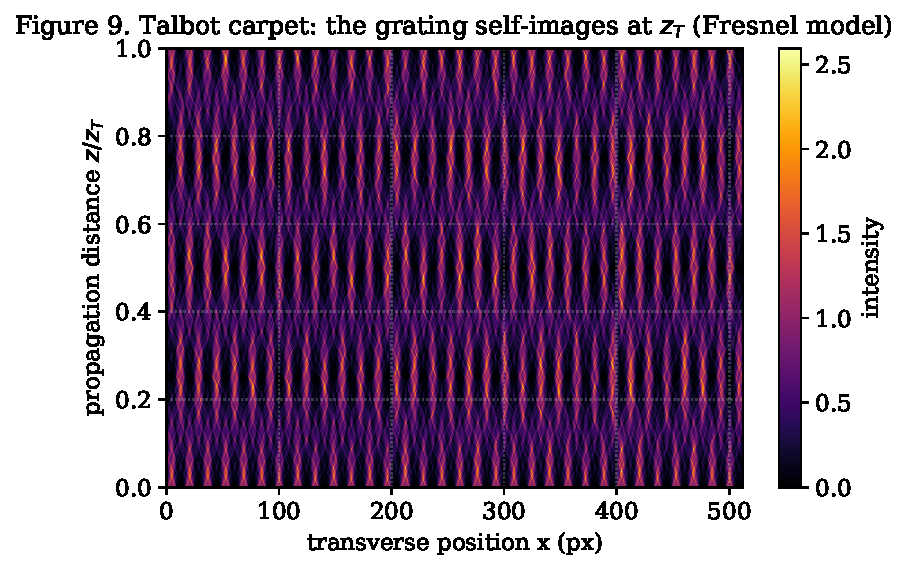
\includegraphics[width=0.7\linewidth]{fig09_talbot.pdf}
\caption{Talbot carpet (Fresnel self-imaging of a periodic display pattern). Self-images recur
at $z_T = 2a^2/\lambda$ and its rational fractions. This classical near-field diffraction is
the wave-optical substrate on which the ``gate'' patterns are encoded and read back --- and it
is fully classical.}
\label{fig:talbot}
\end{figure}

\subsection{Why this is not quantum computing --- the explicit non-claims}
We make the following non-claims prominently, because they are the point of the paper:
\begin{enumerate}
\item \textbf{No single photons.} The OLED emits $\sim\!10^{10}$ photons per frame per region;
every measurement is in the bright, classical regime.
\item \textbf{No entanglement.} Spatial modes of one classical beam can mimic two-qubit algebra
(Spreeuw), but they are separable classical degrees of freedom; there is no nonlocal
correlation and no $2^n$-scaling tensor-product state space.
\item \textbf{No Bell-inequality violation.} A real CHSH test~\cite{chsh} requires
space-like-separated measurements on entangled quanta and the violation of $|S|\le 2$. Our
correlator is local and classical and cannot violate any Bell inequality.
\item \textbf{No no-cloning / no QKD security.} The BB84-labelled demo copies classical patterns
freely; with no single-photon non-cloning it offers \textbf{no} information-theoretic key
security. It is a classical pattern-exchange illustration, not QKD.
\end{enumerate}

\section{A classical lock-in correlator at the display refresh (not a Bell test)}
The one element of the ``quantum'' cluster worth keeping is the phase-sensitive correlator
(repository B11; stages \texttt{chsh}, \texttt{aspect}, \texttt{hom}). The display refresh
(\SI{120}{\hertz}) provides a stable reference modulation. Patterns are emitted with a known
phase/frequency; the captured brightness of each region is demodulated into in-phase and
quadrature components,
\begin{equation}
I_{\cos} = \frac{2}{N}\sum_n y_n \cos(\omega t_n), \qquad
I_{\sin} = \frac{2}{N}\sum_n y_n \sin(\omega t_n),
\end{equation}
with $\omega = 2\pi\,(\SI{120}{\hertz})$, and the angular correlation between two regions is
estimated from $\sqrt{I_{\cos}^2 + I_{\sin}^2}$ and its phase, averaged over many frames with a
$t$-test. This is an ordinary \textbf{classical lock-in amplifier} on a camera stream --- a
useful, narrow technique for pulling weak periodic optical correlations out of noise.

We stress what it is \textbf{not}. Although historically named after CHSH/Aspect, the stage
performs no Bell test. The CHSH bound $|S|\le 2$ for local hidden-variable theories, and its
quantum violation up to $2\sqrt2$, concern measurements on \emph{entangled single quanta} with
space-like separation~\cite{chsh}. Our correlator measures classical intensities of one bright
beam; any ``$S$'' it computes is a classical correlation function bounded trivially by classical
statistics. \textbf{The Bell/quantum interpretation is removed; the lock-in correlator is
retained as a classical method.}

\section{The falsification protocol: the real contribution}
The central risk in any physical-computing claim --- acute when the labels say ``quantum'' ---
is that the apparatus is theatre and the CPU does the work. The Svetoch answer is a
\textbf{mirror-less control}: run the identical software pipeline with the screen facing an open
room, removing the optical return path. If a metric survives, it was a software artifact; if it
collapses, the optics were computing. Applied to the gate emulations, the metrics collapse
(Figure~\ref{fig:qcontrol}, Table~\ref{tab:qcontrol}).

\begin{figure}[ht]\centering
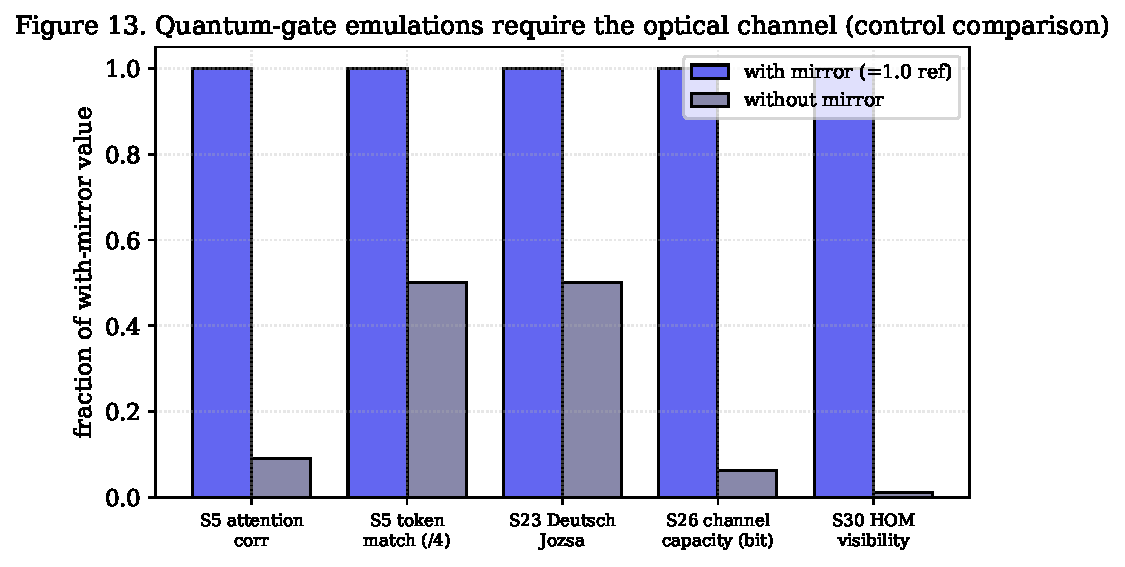
\includegraphics[width=0.82\linewidth]{fig13_quantum_control.pdf}
\caption{Quantum-gate emulation metrics, with mirror vs.\ without mirror (each bar is the
without-mirror value as a fraction of the with-mirror value). Every emulation that needs the
optical channel falls to the noise/coin-flip floor when the mirror is removed.}
\label{fig:qcontrol}
\end{figure}

\begin{table}[ht]\centering\small
\caption{Mirror vs.\ mirror-less control for the gate emulations (documented reference values).
Without the optical channel the emulations reduce to noise or coin-flips.}
\label{tab:qcontrol}
\begin{tabular}{lrrl}
\toprule
Metric (stage) & With mirror & Without mirror & Interpretation\\
\midrule
S5 attention correlation & $1.00$ & $0.09$ & No optical feedback\\
S5 token match & $4/4$ & $2/4$ & Random guessing\\
S2 dot-product correlation & $0.976$ & $-0.41$ & Anti-correlated noise\\
S23 Deutsch--Jozsa & correct & $50\%$ & Coin flip\\
S26 channel capacity & $16$ bit & $1$ bit & Channel gone\\
S30 HOM visibility & $0.056$ & $0.0007$ & $80\times$ lower\\
Dynamic range & $1.42$ & $1.000047$ & No optical channel\\
\bottomrule
\end{tabular}
\end{table}

The Deutsch--Jozsa result is the clearest tell: with the mirror the procedure returns the
correct constant/balanced verdict; without it the verdict is $50\%$ --- a fair coin. A genuine
software computation would be unaffected by removing a mirror. The HOM-labelled ``visibility''
falls $80\times$ to essentially zero, and the channel capacity drops from $16$ bits to $1$ bit
(a single on/off level surviving via stray light). These collapses prove nothing quantum --- only
that there \emph{is} a real classical optical channel and that the emulations use it. That
distinction, demonstrated rather than asserted, is the contribution.

The same control underlies Paper~I (Figure~\ref{fig:control}): removing the mirror drops the
dynamic range $1.42 \to 1.000047$ and weakens white--black contrast by thousands of times across
all stages.

\begin{figure}[ht]\centering
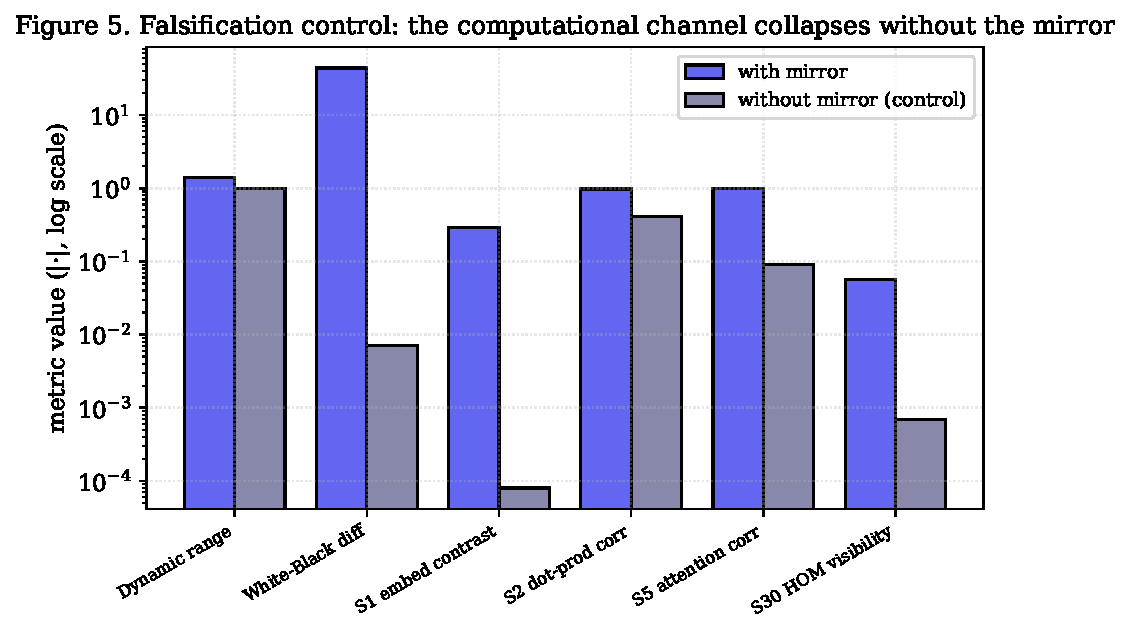
\includegraphics[width=0.84\linewidth]{fig05_control.pdf}
\caption{General falsification control (log scale): for every computational metric the
with-mirror value towers over the mirror-less value. The optical channel, not the CPU, carries
the signal.}
\label{fig:control}
\end{figure}

\section{What survives without the mirror, and why}
We report the survivors honestly, because they bound the contribution.
\paragraph{Shot-noise random numbers are real.} CMOS dark-frame and shot-noise entropy do not
need the mirror; they are a true physical entropy source and pass standard randomness
checks~\cite{trng}. We claim no novelty: extracting randomness from photosensor shot noise has
substantial prior art, and we present it only as the one component that is physically real
\emph{and} mirror-independent.
\paragraph{Monotone stages limp via scattered light.} A weak scattered-light path ($\sim\!0.3\%$
of OLED light reaches the camera through the room and internal cross-talk) lets soft-threshold,
monotone stages partially track their inputs without the mirror --- which is exactly why we do
not count them as evidence of optical computation. A monotone activation correlating with a
monotone input proves only monotonicity, not channel structure.
\paragraph{Spatially resolved stages fail.} Everything requiring real spatial resolution ---
embeddings, dot products, the gate-emulation interference patterns, the lock-in correlations ---
collapses without the mirror (Section~4). That selective failure is the diagnostic we rely on:
real optical effects need the optics; CPU artifacts do not.

\section{Methods}
\textbf{Hardware:} Xiaomi 12 Lite (6.55" AMOLED, $2400\times1080$, \SI{120}{\hertz}, pitch
\SI{63.2}{\micro\meter}; 32\,MP front camera, min.\ focus $\approx$\SI{10}{\centi\meter}); flat
mirror $\sim$\SI{10}{}$\times$\SI{10}{\centi\meter}; gap $d\approx 3\text{--}5$\,cm in a dim
room. Control runs are identical except the mirror is removed and the screen faces an open room.
\textbf{Software:} a dependency-free Python HTTPS server relays Start/Stop and stores runs as
JSON; experiments are browser ES modules. For each gate stage the phone renders the
basis/interference pattern, captures frames with \texttt{getUserMedia}, white-normalizes,
$\gamma$-corrects, computes the stage metric (interference contrast, $\arg\max$ verdict, lock-in
$I_{\cos}/I_{\sin}$, HOM visibility, capacity), and posts results; the lock-in demodulation uses
the \SI{120}{\hertz} refresh as reference and aggregates many frames with a $t$-test.
\textbf{Figures:} produced by \texttt{papers/scripts/make\_figures.py}; real-data figures use a
reference run (2026-06-06); the Talbot carpet (Figure~\ref{fig:talbot}) is a wave-optics model,
labelled as such.

\section{Discussion}
The value of these experiments is as a \textbf{teaching and analogue platform}, not as a quantum
computer. They let a student build the algebra of Hadamard, QFT, Grover and Deutsch--Jozsa from
brightness patterns and interference on hardware they already own, and --- crucially --- test
whether the apparatus does anything physical by removing the mirror. The discipline of the
falsification control transfers well beyond this project: any claim that ``a physical substrate
computes $X$'' should come with a null configuration in which the substrate is removed and the
metric is shown to collapse.

\paragraph{Explicit non-claims (restated).} No single photons; no entanglement; no
Bell-inequality violation; no no-cloning and hence no QKD security; no quantum speed-up. The
``QFT-by-diffraction'' has heavy Fourier-optics prior art and is not a true focal-plane transform
on this device. The shot-noise TRNG is physically real but has prior art. The CHSH/Aspect-labelled
stage is a classical lock-in correlator, not a Bell test, and its quantum interpretation is
withdrawn.

\paragraph{Limitations.} The classical encoding pays at least linearly in the number of emulated
qubits, so the analogue does not scale; ambient light, vibration and mirror quality degrade
contrast; the pass thresholds are device-specific; cross-device reproducibility is an open
validation shared with the rest of the series.

\section{Conclusion}
A smartphone and a mirror can faithfully \textbf{emulate the linear algebra of quantum gates with
classical wave optics} --- and a mirror-removal control proves these are classical optical effects, not CPU
theatre and not quantum computation. We have set out exactly what is and is not being computed,
retained the one defensible measurement primitive (a classical lock-in correlator) on honest
terms, noted the real-but-prior-art shot-noise TRNG, and given the falsification protocol whose
collapse numbers (HOM $0.056\to0.0007$, Deutsch--Jozsa $\to50\%$, capacity $16\to1$ bit) are the
project's honesty test. We publish this framing openly so the record is unambiguous: an honest
classical analogue, not a quantum claim.

\paragraph{Data and code.} \href{https://github.com/infosave2007/svetoch}{github.com/infosave2007/svetoch}; related VMF/NVG theory: \href{https://github.com/infosave2007/vmf}{github.com/infosave2007/vmf}
(Apache-2.0); reference-run data under \texttt{examples/} and \texttt{papers/scripts/}.
\paragraph{Priority note.} Released as a defensive publication to establish authorship and date
of disclosure --- in particular the honest classical-analogue framing and the falsification
protocol; the author has elected not to seek patent protection.

\begin{thebibliography}{9}\small
\bibitem{spreeuw} R. J. C. Spreeuw, ``A classical analogy of entanglement,'' \emph{Found. Phys.} \textbf{28}, 361 (1998).
\bibitem{goodman} J. W. Goodman, \emph{Introduction to Fourier Optics}, 3rd ed., Roberts \& Company, 2005.
\bibitem{chsh} J. F. Clauser, M. A. Horne, A. Shimony, R. A. Holt, ``Proposed experiment to test local hidden-variable theories,'' \emph{Phys. Rev. Lett.} \textbf{23}, 880 (1969).
\bibitem{talbot} H. F. Talbot, ``Facts relating to optical science No.\ IV,'' \emph{Phil. Mag.} \textbf{9}, 401 (1836).
\bibitem{trng} M. Stip\v{c}evi\'c, B. Medved Rogina, ``Quantum random number generator based on photonic emission in semiconductors,'' \emph{Rev. Sci. Instrum.} \textbf{78}, 045104 (2007).
\bibitem{solli} D. R. Solli, B. Jalali, ``Analog optical computing,'' \emph{Nat. Photon.} \textbf{9}, 704 (2015).
\end{thebibliography}

\svetochfooter
\end{document}
